\documentclass[twocolumn,showpacs,preprintnumbers,prd,superscriptaddress,nofootinbib]{revtex4}
 %%\pdfoutput=1
\usepackage{epsfig}
\usepackage{graphicx}
\usepackage{amsmath,amssymb,amsfonts}
\usepackage{array}
\usepackage{url}
\usepackage{hyperref}
\usepackage{lineno}
\usepackage{xspace}


% lineno works with the two commands below, of 'linenumbers'
%\usepackage{latexsym}
\usepackage{graphics}
\usepackage{graphicx}
\usepackage{xcolor}
%\usepackage[pagewise]{lineno}
%%%%\usepackage[switch]{lineno}
%%%%\def\linenumberfont{\footnotesize}
% etc
%
%

\begin{document}
\def\jour#1#2#3#4{{#1} {\bf#2}, #4 (19#3)} %% #4}
\def\jou2#1#2#3#4{{#1} {\bf#2}, #4 (20#3)} %% #4}
\def\PRL{{Phys. Rev. Lett. }}
\def\EPJA{{Eur. Phys. J.  A }}
\def\EPL{{Europhys. Lett.}}
\def\PRv{{Phys. Rev. }}
\def\PRC{{Phys. Rev.  C }}
\def\PRD{{Phys. Rev.  D }}
\def\JAP{{J. Appl. Phys. }}
\def\AJP{{Am. J. Phys. }}
\def\NIMA{{Nucl. Instr. and Meth. Phys. A }}
\def\NPA{{Nucl. Phys. A }}
\def\NPB{{Nucl. Phys.  B }}
\def\NPBP{{Nucl. Phys.  B (Proc. Suppl.) }}
\def\NJP{{New J.  Phys. }}
\def\EPJC{{Eur. Phys. J.  C }}
\def\PLB{{Phys. Lett. B }}
\def\PHY{{Physics }}
\def\MPLA{{Mod. Phys. Lett. A }}
\def\PRp{{Phys. Rep. }}
\def\ZPC{{Z. Phys. C }}
\def\ZPA{{Z. Phys. A }}
\def\PPNP{{Prog. Part. Nucl. Phys. }}
\def\JPG{{J. Phys. G }}
\def\CPC{{Comput. Phys. Commun. }}
\def\APP{{Acta Physica Pol. B }}
\def\AIP{{AIP Conf. Proc. }}
\def\JHEP{{J. High Energy Phys. }}
\def\PSC{{Prog. Sci. Culture }}
\def\NCim{{Nuovo Cim. }}
\def\SNC{{Suppl. Nuovo Cim. }}
\def\SJNP{{Sov. J. Nucl. Phys. }}
\def\SPJ{{Sov. Phys. JETP }}
\def\JLet{{JETP Lett.}}
\def\PTP{{Prog. Theor. Phys. }}
\def\PTPS{{Prog. Theor. Phys. Suppl. }}
\def\IANSF{{Izv. Akad. Nauk SSSR: Ser. Fiz. }}
\def\JPCS{{J. Phys. Conf. Ser. }}
\def\AHEP{{Adv. High Energy Phys. }}
\def\IJMPE{{Int.  J. Mod. Phys. E }}
\def\ARNPS{{Ann. Rev. Nucl. Part. Sci. }}

%%\def\jour#1#2#3#4{{#1} {\bf#2} (19#3) #4}
%%\def\jou2#1#2#3#4{{#1} {\bf#2} (20#3) #4}
\def\ct{\cite}
\def\sNN{\sqrt{s_{N\!N}}}
\def\sNNq{s_{N\!N}}
\def\sppq{s_{pp}}
\def\spp{\sqrt{s_{pp}}}
\def\eNN{\varepsilon_{N\!N}}
\def\pbp{{\bar p}p}

\def\col{Collab.}
\def\bi{\bibitem}
\def\ea{{\sl et al.}}
\def\eg{{\sl e.g.}}
\def\vrs{{\sl vs.}}
\def\ie{{\sl i.e.}}
\def\va{{\sl via}}
%
\def\nopar{\noindent}
%\def\app{${\bar {\rm p}}{\rm p}$}
%\def\see{\sqrt{s_{\rm ee}}}
%\def\ep{$\rm{e}^+\rm{e}^-$}
%
%\def\vs{\vspace*}
%\def\hs{\hspace*}
\def\bi{\bibitem} 
%\def\fig{Fig}
%\def\sect{Sect.}
 %%\def\col{Collaboration}
%\def\col{Collab.}
%\def\lss{\pm\,\pm}
%\def\al{\langle}
%\def\ar{\rangle}
%\def\lssim{\leqslant}
%\def\geq{\geqslant}  
%
\def\lssim{\stackrel{<}{_\sim}}
\def\gtsim{\stackrel{>}{_\sim}}
%\def\lssim{\lesssim}
%\def\gtsim{\gtrsim}
%

% \linenumbers % uncomment to get rid of line numbering !!!!
%\runningpagewiselinenumbers

\title{
  Effective-energy universality 
  %%%%picture 
  approach 
 %%%description of 
 describing
 total multiplicity 
 centrality  dependence 
 %%%%of multiplicities   
 in 
 %%%GeV to TeV 
 heavy-ion collisions  
  %%%%spanning GeV to TeV energies
}
\author{Edward K. Sarkisyan-Grinbaum}
%%%\email {sedward@cern.ch}
\email {Edward.Sarkisyan-Grinbaum@cern.ch}
\affiliation{Experimental Physics Department, CERN, 1211 Geneva 23, 
Switzerland}
\affiliation{Department of Physics, The University of Texas at
Arlington, Arlington, TX 76019, USA}
\author{Aditya Nath Mishra}
\email {Aditya.Nath.Mishra@cern.ch}
\affiliation{Instituto de Ciencias Nucleares, Universidad Nacional 
Autonoma de Mexico, Mexico City, 04510, Mexico}
\author{Raghunath Sahoo}
\email{Raghunath.Sahoo@cern.ch}
\affiliation{Discipline of Physics, School of Basic Science, Indian
Institute of Technology, Indore 452020, India}
\author{Alexander S. Sakharov}
\email{Alexandre.Sakharov@cern.ch}
\affiliation{Experimental Physics Department, CERN, 1211 Geneva 23, 
Switzerland}
\affiliation{Department of Physics, New York University, New York, NY
10003, USA}
\affiliation{Physics Department, Manhattan College, Riverdale, NY 10471,
USA}

%
 \begin{abstract} 
 The recently proposed participant dissipating effective-energy approach  
is applied to describe
    %%%the recent measurements of  
  the dependence on centrality 
   %%%, or on the number of nucleon participants, 
 of the  multiplicity 
   %%%% the midrapidity density 
  of charged particles measured in heavy-ion collisions at the collision 
 energies
   %%%of several orders of magnitude, 
   %%%up to 200 
   %%%of about 20 
   %%%GeV  at RHIC to 
  up to the 
 %highest 
 LHC energy of 5 TeV.
 The effective-energy approach relates multihadron production in different 
types of collisions, by combining, under the proper collision energy 
scaling,
   %%% of the collision energy,
  the constituent quark picture with Landau relativistic hydrodynamics.
   %%% is 
 %%%investigated
 %%%within 
 %%%This approach,  
  The measurements are shown to be well described in terms of the 
centrality-dependent effective energy of participants 
 %%% along with a given 
   and an explanation of the differences in the measurements at RHIC and 
LHC are given by means of the recently introduced hypothesis of the 
energy-balanced limiting fragmentation scaling.
 A similarity between the centrality data and the data from most central 
collisions is 
 proposed 
 %%%shown 
 pointing to the central character of participant 
interactions 
 independent of 
  %%%%at different
  %%%types of 
     centrality.
  The findings complement 
    %%%those from
  our 
 earlier 
 %%%recent 
 % investigations 
 studies
 of the similar midrapidity pseudorapidity 
density measurements 
       extending the 
 description to the full pseudorapidity range 
 in view of 
 %%%driven by the participant effective-energy
 %%%and a possible change of 
  %%%hadroproduction mechanism moving from GeV to TeV energies are
   %%%suggested
   %
  %%%based on 
  the 
   %considered 
 similarity 
  of multihadron production
   %%%process 
 in 
  %%(anti)proton-proton
 nucleon interactions 
 and heavy-ion collisions. 
   %%driven by the centrality-dependent effective energy 
     %%of participants.

\pacs{25.75.Dw, 25.75.Ag, 24.85.+p, 13.85.Ni}
 \end{abstract}

\maketitle

%\nopar
 %\section*{Introduction}
 %\label{intro}
 %%{\bf 1. } 
 %%%% Recently, we have shown \ct{edward502} 
 %%%%that the centrality dependence of the midrapidity 
 %%%% pseudorapidity density in heavy-ion collisions 
  %%% at 
 %%%% in the range of 
%%% the center-of-mass (c.m.) energy, $\sNN$, 
 %%%%  spanning GeVs to TeVs,
  %%%from few 
   %%%some
  %%%GeVs up to 
  %%% $\sim \!5$~TeV
  %%%about 5 TeV 
  %%%% is well described in the framework of the approach of the 
 %%%% dissipating 
 %%%% energy of constituent quark participants, or, for brevity, the 
 %%%% effective-energy approach, 
 %%%%
 %%%% Within this description, 
   %%%In describing the multiplicities, we provide
 %%%%an explanation of the so-called RHIC ``puzzle'', 
 %%%%namely of the difference between the nucleon-participant-normalized 
 %%%%total multiplicity independence of centrality  
 %%%%and the midrapidity pseudorapidity density  increase with 
 %%%%centrality, is suggested. 
 %%%%This difference is found to be 
 %%%is 
 %%%%taken into account by introducing the energy-balanced limiting 
 %%%%fragmentation scaling allowing to well describe the multiplicity 
 %%%%data and 
 %%%%the pseudorapidity spectra independent of centrality. No such 
 %%%%a difference is measured at the LHC at TeV 
 %%%%energies, where both the normalized midrapidity density and 
 %the 
 %%%%multiplicity are observed to decrease with the centrality, as 
 %%%%indeed is expected within the effective energy approach.
   %% and indicating a possible change of 
   %%the regime of multiparticle production in heavy-ion collisions 
   %%at TeV energies.    

Recently, the measurements 
of the
centrality dependence of the (mean) total multiplicity of charged 
 particles in PbPb collisions 
 at 
 %%the c.m. energy 
 %%per 
 %%nucleon
 %ever reached, namely at 
the center-of-mass (c.m.) energy
 $\sNN=5.02$~TeV
 %%, 
 %%%%%%the highest collision energy ever reached, 
 %%of 5.02~TeV, 
 have been reported 
 by
 ALICE 
\ct{alice-mult5}.
 %{\bf
 Here, we describe these measurements in the framework of the dissipating 
energy of constituent quark participants, or, for brevity, the 
effective-energy approach, proposed by two of us in \ct{edwarda,edward}. 
Exploiting a 
concept of centrality-dependent effective energy on nucleon participants 
\ct{edward2},
 one demonstrates that the 5.02 TeV ALICE measurements can be well 
accommodated by the above approach and thus complements the results of our 
findings \ct{edward502} 
 of 
 %an excellent 
 a very good
description of the data on the measurements of the 
midrapidity pseudorapidity densities in nucleus-nucleus collisions within 
the energy range up to 5.02 TeV, provided that the the total multiplicity 
is the critical variable for obtaining the information on the 
multihadron production 
dynamics \ct{multrev,book,pprev}.  
 %} %%%bf ends
 
 %In the study presented here, we show that these measurements 
 %are 
 %%%also 
  %%%% is 
 %well described in the framework of the approach of the 
 %dissipating 
 %energy of constituent quark participants, or, for brevity, the 
 %effective-energy approach, 
 %%%% well described 
 %%%% in the picture of the  
%%%%  participant dissipating effective-energy approach,
 %proposed by two of us \ct{edwarda,edward}  and
 %exploiting a concept of centrality-dependent effective energy of 
 %nucleon participants \ct{edward2}.
 %%%%In this paper we 
 %The study extends our earlier investigations 
 %\ct{edwardPRD}, where we 
 %have  shown 
 %that within the effective-energy approach one well describes 
 %the 
 %total (mean) multiplicity data and the pseudorapidity distributions 
 %in
 %heavy-ion collisions up to 2.76 TeV collision energy. 
 %Meantime, the results of 
 %this  study 
 %extends
 %%%extending  
 %complement
 %our findings  \ct{edward502} 
 %of a good description of the data
 %%%from 
 %of  the midrapidity
 %pseudorapidity  densities, measured in nucleus-nucleus collisions 
 %in the entire available energy range up  to 5.02 TeV,
 %by a description of the data 
 %%%to 
 %in the full pseudorapidity range, 
  %%%and so to
  %then  
  %the total multiplicity, 
   %%%%the latter representing
  %a variable 
 %providing crucial information of the multihadron production dynamics 
 %\ct{multrev,book,pprev}.  
 

 %{\bf
 Let us give a brief description of  the effective-energy approach.
 Within this approach, 
 %one
 which    
 interrelates different types of collisions \ct{edwarda},
  %This approach interrelates the particle 
  %production process in different types of 
 %collisions \ct{edwarda}, 
 %% Within its 
 %%the PDE 
 % such a 
 %%picture of the participant dissipating energy,   
 %approach 
 %%the effective-energy approach 
 the particle production process 
 %is quantified 
is quantified
 in 
 terms of the 
amount of {\it effective} energy
deposited 
 %%by interacting constituent quark participants 
into the small
 Lorentz-contracted volume 
 which is 
formed at the early stage of a 
collision.
  Then, the
 whole process of  the particle production
 %a collision  
  is 
 %then 
 considered
 %represented 
  as the expansion of an initial state 
  and the subsequent break-up into particles.  
This 
 picture
  resembles 
the Landau
 relativistic
 %% phenomenological 
 hydrodynamic model
 %approach
 %%% to   
 of 
 multiparticle production 
 %in relativistic particle interactions 
 \ct{Landau}.
 %% , which was found to be in a  good agreement with 
 %% the multiplicity data in particle and nuclear collisions 
 %% in  the wide energy range \ct{Landau-difint}. 
 In the meantime, the effective-energy approach 
 considers 
the Landau 
hydrodynamics 
 being
 %which 
 %is 
 treated 
 % employed 
 in the framework of constituent (or dressed) quarks, in 
 accordance with the additive quark model \ct{additq,constitq}.
 This makes the secondary particle  production 
to be  basically driven by  the amount of the 
 initial 
 %% {\it effective}  
 %deposited  by
 energy 
 of 
 constituent quarks 
 %% 
 pumped into the Lorentz-contracted 
 overlap 
 region
 of colliding objects.
 %. In
 Then, in $pp/\pbp$ collisions, a single constituent quark from  
 each nucleon is 
 assumed
 %considered
  to   contribute
 %% take part 
 in a collision.
 %%  and the  
 The remaining quarks
 %rest 
 are treated as spectators. 
  The spectator quarks 
 %%and 
 do not participate in the 
 %% secondary 
 particle 
 %% 
 production, while 
 %they  
 result
   into 
 %in 
 %%%% a 
 formation of leading particles 
  and 
 carrying away a  significant part of the collision energy.
 %%  of a collision.
  Thus, 
  the effective energy for
  multiparticle production in  $pp/\pbp$ collisions is the energy of 
  a single quark pair   interaction,
  i.e. represents 1/3 of the entire nucleon energy.
 In collisions of nuclei, however, due to the large size of the 
nucleus and the long travel path inside the nucleus, more than one quark 
per nucleon can interact. 
 %On the contrary, in
 In 
 the most central (head-on) heavy-ion collisions, 
 %%% on the contrary,  
 where the colliding nuclei are almost fully overlapped, 
 %% with 
 all three constituent quarks from each of the participating nucleons 
 may interact 
  and deposit their energy 
 into the collision zone.
 %are %considered 
 %treated 
 %to contribute
  %% nucleon.
 %which 
  Then
 % makes  
 % so that 
the whole energy of the 
 %% colliding 
 nucleons 
 %% (participants) 
 %% is considered to be 
 becomes available for the 
 %% secondary
 particle production.  
 %Thus, 
  Within this picture,
 %% one  expects 
 %that 
 the 
 %% results 
 %% for 
 bulk 
 %%%%production 
 measurements
 %% observables 
 %measured  
 in 
 %%%% from 
 head-on heavy-ion collisions 
 %%%%% 
 at 
 %%%%% the c.m. energy per nucleon, 
 $\sqrt{s_{NN}}$
 %%%% , 
 are 
 %%  treated
 expected 
 to be similar to 
  those from
 %%% that 
 %% the  
 %%% in 
 $pp/\pbp$ collisions 
 %%%% 
but at 
 %%  corresponding to at 
 %the 
 %%%
  a
 three times larger 
 %%%%,
 % properly
 %%%% correspondingly scaled  
 c.m. energy $\sqrt{s_{pp}}$, 
 %%%%scaled by a factor of 3,  
  i.e. 
  %%\ie\ 
  % taken 
 at 
 $\sqrt{s_{pp}} \simeq 
 3\sqrt{s_{NN}}$.
 Let us stress here that the effective-energy approach is considered 
being applied to the bulk variables, while it is well understood that 
collective effects such as elliptic flow, correlations would provide 
furter important details but to be addressed in separate studies.

 Combining 
 within the above consideration
 %%Being put together, 
 the 
 %above-discussed 
 two contributing 
 ingredients, namely the 
 %% of the 
 constituent quark picture and  the pseudorapidity density 
 from the Landau hydrodynamics, 
 %}%%%%%%%%%%%%bf ends 
%%%%
  one obtains 
 %%lead to 
 the relationship between 
 the 
charged particle rapidity density
per participant pair, 
 $\rho(\eta)=(2/N_{\rm{part}})dN_{\rm{ch}}/d\eta$, 
in heavy-ion 
 collisions  and in  $pp/\pbp$  
 interactions \ct{edwardPRD}:
 %%%collisions:

 \begin{eqnarray}
 &\!\!\!\!\! &    
 \nonumber
\frac{\rho(\eta)}{\rho_{pp}(\eta)}\!=\!
\frac{2N_{\rm{ch}}}{N_{\rm{part}}\, N_{\rm{ch}}^{pp}}
\, \sqrt{\frac{L_{pp}}{L_{N\!N}}} \,
 \exp\! \left[ \frac{\eta^2}{2} \left(
 \frac{1}{L_{pp}}
 - 
 \frac{1}{L_{N\!N}} 
 \right) \right] \, , \\
 &\!\!\!\!\! &    
 %% & &   
 \spp=3\sNN\, .
 \label{rapdistf}
 \end{eqnarray}
 %
 %---
 %%  %Eqn.1
 %% \begin{equation}
 %% \frac{\rho(0)}{\rho_{pp}(0)} = 
 %% \frac{2N_{\rm{ch}}}{N_{\rm{part}}\, N_{\rm{ch}}^{pp}} 
 %% \, \sqrt{\frac{L_{pp}}{L_{N\!N}}} \, ,\:\:\:\:\:
 %% \spp=3\sNN\, .
 %% \label{eqn1}
 %% \end{equation}
 %
 Here, 
 $N_{\rm{ch}}$ and 
 $N_{\rm{ch}}^{pp}$ are the (total) mean multiplicities in nucleus-nucleus 
and nucleon-nucleon collisions, respectively, and $N_{\rm {part}}$ is the 
number of nucleon 
participants. The relation of the pseudorapidity density 
and the 
mean multiplicity is applied in its Gaussian form as obtained in Landau 
hydrodynamics. The factor $L$, which is related to the Lorentz contraction of the system,
 is defined as $L = {\ln}({\sqrt{s}}/{2m})$. 
According to the approach considered, $m$ is the proton mass, $m_{p}$, in 
nucleus-nucleus collisions and
 represents the constituent quark mass ($m_{q}$) in $pp/\pbp$ collisions 
 %which is 
 set
 to  $\frac{1}{3}m_{{p}}$.
 %%  In Eq.(\ref{eqn1}), 
 %the Gaussian form of 
 %% the 
 %%Such an universality was found to correctly predict \ct{edward} the 
 %%value of the midrapidity density in $pp$ interactions measured at LHC 
  %%TeV energies \ct{CMSwe}.

 %%%% Evolving 
 % Solving Eq.~(\ref{rapdistf}) for the multiplicity $N_{\rm{ch}}$ at a 
 %given midrapidity density pseudorapidity $\rho(\eta\! \approx\! 0)$ at 
 %$\sqrt{s_{NN}}$, and for the rapidity density $\rho_{pp}(0)$ and the 
 %multiplicity $N_{\rm{ch}}^{pp}$ at $3 \sqrt{s_{NN}}$, one finds:

 %Solving Eq.~(\ref{rapdistf}) at midrapidity ($\eta\! \approx\! 0$) one 
 %finds:
 At the midrapidity, $\eta\! \approx\! 0$,  Eq.~(\ref{rapdistf}) 
simplifies  to: 

\begin{eqnarray}
\nonumber
\frac{\rho(0)}{\rho_{pp}(0)}&=&
\frac{2N_{\rm{ch}}}{N_{\rm{part}}\, N_{\rm{ch}}^{pp}} 
\sqrt{\frac{L_{pp}}{L_{N\!N}}} \ , \\
\sNN&=&\spp/3 \, .
 \label{eqn2}
\end{eqnarray}
 %
Taking into account that $L_{pp} = \ln \left( \spp/2m_q \right)$ 
 and  $L_{N\!N} = \ln \left( \sNN/2m_p \right)$ and setting
  %%$m_q=\frac{1}{3}m_p$ 
  $m_q=m_p/3$ 
 and  $\spp=3\sNN$, one gets for Eq.~(\ref{eqn2}):

\begin{eqnarray}
\nonumber
\frac{\rho(0)}{\rho_{pp}(0)}&=&
\frac{2N_{\rm ch}}{N_{\rm part}\, N_{\rm ch}^{pp}} 
\sqrt{1 -
\frac{4\, \ln 3}{\ln \left( 4m_p^2/s_{NN}\right) }} \ ,  \\ 
\sNN&=&\spp/3 \, .
\label{eqn3}
\end{eqnarray}
\nopar

Solving Eq.~(\ref{eqn3}), for the multiplicity $N_{\rm{ch}}$ at a given midrapidity density  pseudorapidity $\rho(\eta\! \approx\! 0)$ at $\sqrt{s_{NN}}$, and for the rapidity density  $\rho_{pp}(0)$ and the multiplicity $N_{\rm{ch}}^{pp}$ at $3 \sqrt{s_{NN}}$, one finds:

\begin{eqnarray}
\nonumber
\frac{2N_{\rm{ch}}}{N_{\rm{part}}}  &=&
N^{pp}_{\rm ch} \,
\frac{\rho(0)}{\rho_{pp}(0)} \,
\sqrt{1-\frac{2 \ln 3}{\ln\, (4.5 \sNN/m_ p)}}\ ,  \\
	    \sNN&=&\spp/3 \, .
\label{eqn4}
\end{eqnarray}
\nopar




 In the 
 further development  \ct{edward2}, 
 %%% as outlined below, 
 one 
 considers 
  %%% treats  this  dependence 
 %%the obtained relation,  
 this dependence 
 %%Eq. (\ref{eqn1}) 
 in
terms of centrality.
 %%%% \ct{edward2}. 
 %{\bf 
 The centrality 
 %considered to characterize 
 %% The most central collisions 
 %% correspond therefore to the lowest centrality while the larger
 %% centrality 
 %define 
 %% to the more peripheral collisions. 
 %% The centrality 
 is closely 
related to the number of nucleon participants
 determined using Monte Carlo Glauber calculations, 
 %Hence,
  so that 
  the largest number of participants 
  contribute to the most central heavy-ion collisions. 
 %% .
 % \ct{GlauberMCrev}. 
 In the meantime, the centrality is 
 regarded as the degree  of the overlap of the  volumes of the 
 two colliding  nuclei, 
 %determined 
 characterized  by the impact parameter.
 The smaller the impact parameter (more central collisions), the
larger is  the overlap zone.
 Considering the 
 volumes of the colliding nuclei projected onto the
overlapped area 
 as 
being populated by the number of 
participants depositing their energy into the 
Lorentz-contracted volume of the early stage collision zone, the 
centrality, in the participant effective-energy approach, can 
  be  
 %%thus 
 related to the amount of the energy 
 released
 %, 
 %%in the framework of the effective-energy approach,  
 for 
 particle production, 
 %%\ie\
 i.e.   to the effective energy, $\eNN$, of  
the participants.
 %, which, 
 %The latter, i
 %} %%%%bf ends here %% 
 Then
 this effective energy 
 can be 
defined as 
a fraction of the c.m. energy available in a collision according to the 
centrality, $\alpha$:
 %%%%\footnote{ [was about centrality interval, see just after the Eq.]
 %%}
 %
 \begin{equation}
\eNN = \sqrt{s_{NN}}(1 - \alpha).
\label{Eeff}
\end{equation}
 %{\bf 
  One has to note that this relation is satisfied for all but most 
peripheral collisions, where no overlap zone can be actually defined 
and the collisions rather resemble diffractive interactions of 
nucleons, 
so no scale factor 1/3 to be applied anymore. 
 %} %%%%bf 

  Conventionally, the data are divided into 
 classes of centrality, or 
  centrality intervals, so that $\alpha$ is the average 
 centrality per 
 %%for the 
 centrality interval, \eg\ $\alpha = 0.25$ for the centrality 
  interval of 
 20--30\% centrality.

Then, for non-central collisions, 
 %%after taking into account the energy scaling,
 %Eq.~(\ref{eqn1})  
 Eq.~(\ref{eqn4})  
 reads
 
\begin{eqnarray}
& &
\nonumber
\frac{2N_{\rm{ch}}}{N_{\rm{part}}}  =
  N^{pp}_{\rm ch} \,
   \frac{\rho(0)}{\rho_{pp}(0)} \,
  \sqrt{1-\frac{2 \ln 3}{\ln\, (4.5\ \eNN /m_ p)}}\,,  \\
& &    \eNN=\spp/3 \, .
  \label{pmultc}
\end{eqnarray}
  \nopar
 %
 considering
 %for 
 central 
 %%nucleus-nucleus 
collisions of nuclei
  at 
 %%measured 
 the effective c.m.  energy 
 $\eNN$. Here
 %%where
 %%$N_{\rm{ch}}$
 %%$\rho(0)$ 
 %%is  
 %the  multiplicity
 %%the midrapidity density 
  %%in 
  %%at  $\sNN=\eNN$, 
 %%and 
 $\rho_{pp}(0)$ 
 and 
 $N_{\rm{ch}}^{pp}$  
 are
 %%%%
 %% the midrapidity density 
 %%%%
 %%  and the multiplicity 
 taken 
 from  $pp/{\bar p}p$ 
 data
 %interactions
 at  $\spp=3\, \eNN$.
 

Let us note that each of the scalings introduced by  Eqs.~(\ref{eqn4}) and 
~(\ref{Eeff}) 
regulates a particular physics ingredient 
 %%used in the 
 of the
 modelling within the 
participant dissipative effective-energy  
approach. The scaling embedded in Eq.~(\ref{eqn4}) reflects the 
constituent 
quark picture and then reveals a similarity of multihadron 
production in hadronic and 
nuclear collisions. The scaling driven by Eq.~(\ref{Eeff}) addresses the 
energy budget effectively retained in the most central collisions while 
defining the energy availability for the global variables in non-central 
collisions.

 %%In fact, 
 %%%% To note is that 
 %%%% each of the scalings described by Eqs.(\ref{pmult}) and 
 %%%% (\ref{Eeff}) regulates a particular physics ingredient used 
 %%%% in the 
 %%%% modeling of the 
 %% PDE 
 %%%% dissipating effective-energy approach. The scaling 
 %%%% %introduced by Eq.(\ref{pmult}) 
 %%%% embeds the constituent quark model, which leads to 
 %%%% establishing a 
 %%%% similarity between hadronic and nuclear collisions. The 
 %%%% scaling 
 %%%% driven by 
 %%%% Eq.(\ref{Eeff}) is
 %%%% addressed
 %% appealed 
 %%%%% to define the energy budget
 %%%% effectively retained for multiparticle production in the 
 %%%% most central collisions while 
 %%to determine 
 %%%% determing the global variables 
 %% obtained 
 %%%% from 
 %% centrality data. 
 %%%%% non-central collisions.
 %%%% This approach is also found to well reproduce the 
  %%%%% mean multiplicity measurements while revealing 
 %%%% a new type of scaling for 
 %%% non-central collisions \ct{edwardPRD}.
 %%\\


%Fig.1
%\begin{figure}
\begin{figure*}%\sidecaption
 \begin{center}
%\resizebox{0.5\textwidth}{!}{%
\resizebox{0.65\textwidth}{!}{%
%  \includegraphics{Fig1}}
  %%\includegraphics{rap0npart5020_w}}
  \includegraphics{Figure1.eps}}
  %%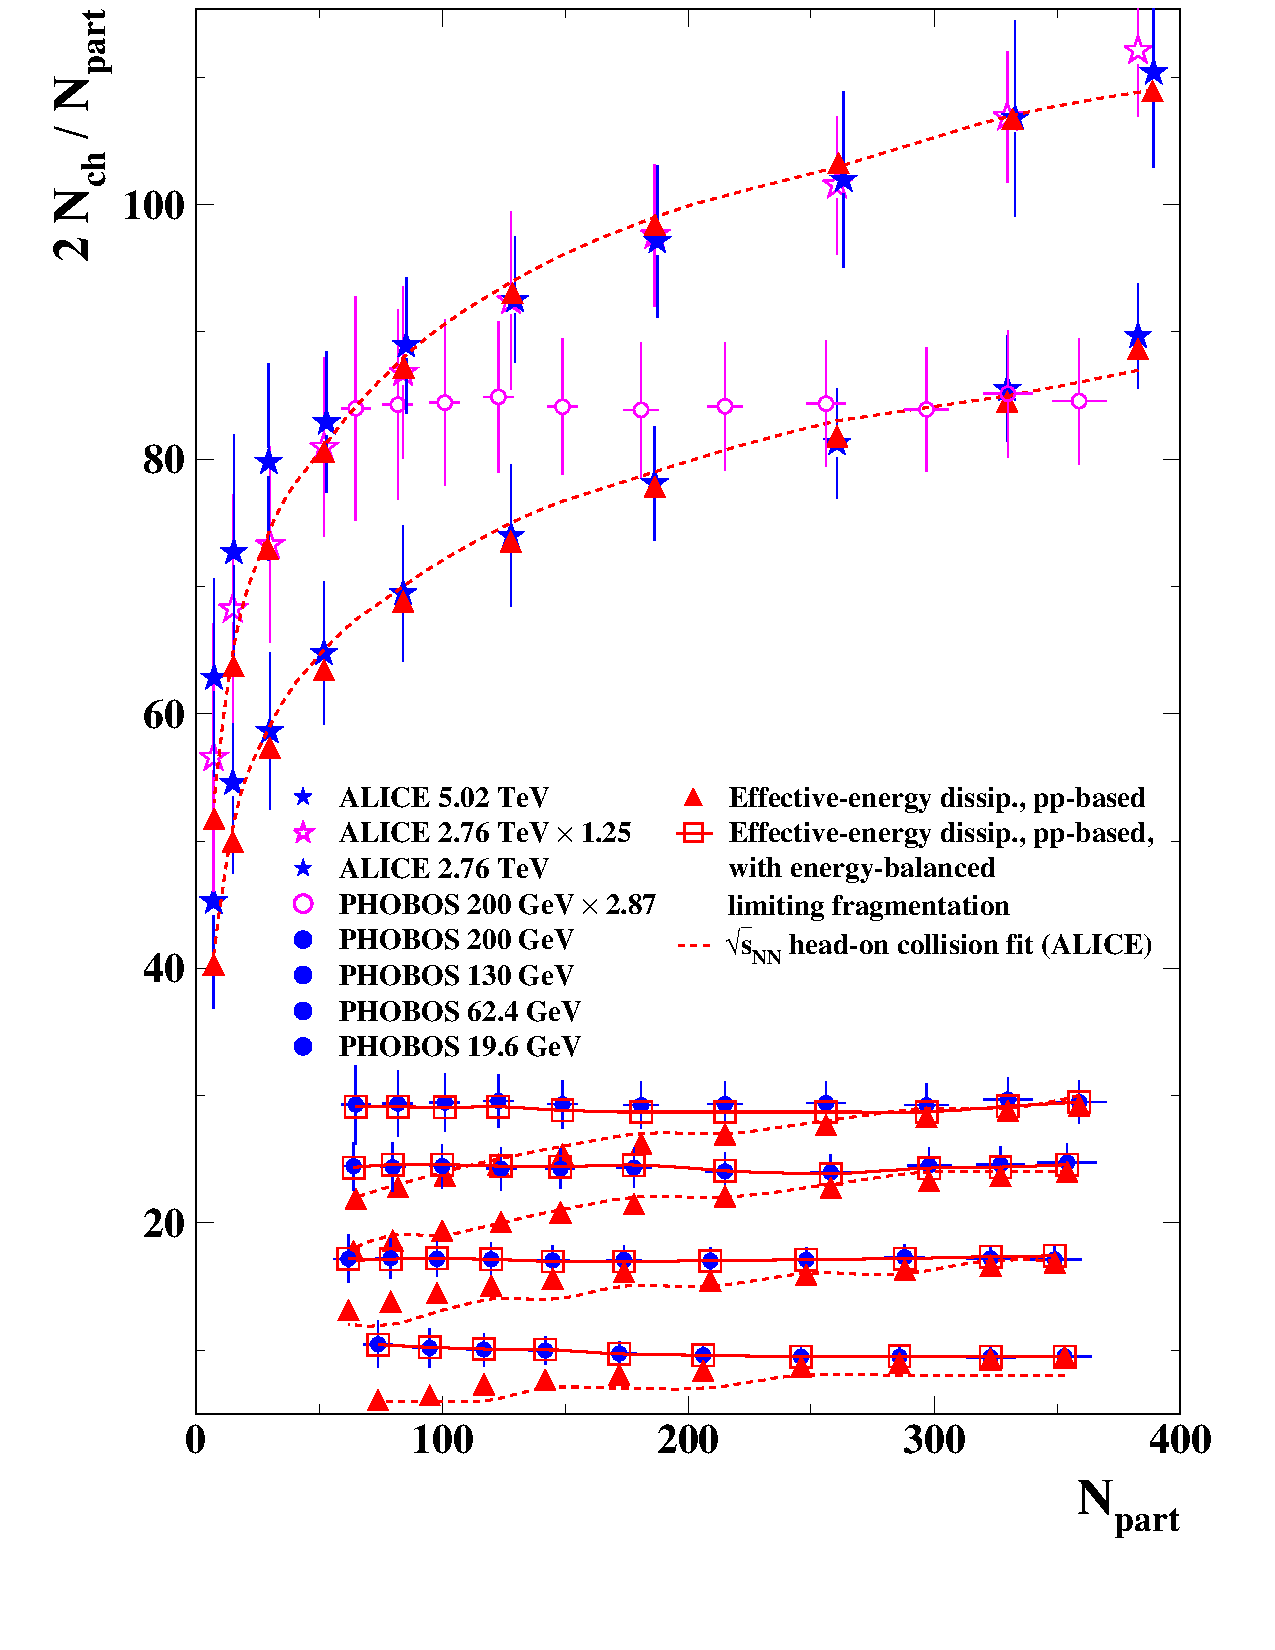
\includegraphics{Figure1.pdf}}
 \end{center}
% \vspace*{-1.5cm}
\caption{
The
 charged particle
 mean multiplicity
per participant
pair as a function of the number of participants, $N_{\rm part}$.
 The
solid
 stars show the dependence measured in 
PbPb collisions at the LHC by the ALICE experiment at $\sNN=2.76$~TeV
\ct{alice-mult2} and 5.02 TeV \ct{alice-mult5}, 
and the
 solid
 circles show the 
 measurements from 
 AuAu collisions at RHIC  by
the PHOBOS experiment at $\sNN=19.6, 62.4, 130$ and 200~GeV
\ct{phobos-all} (the symbols indicate $\sNN$ 
increasing
bottom to top). 
 The
 triangles show the calculations
by Eq.~(\ref{pmultc}) using $pp/\pbp$ data within the participant 
dissipating effective-energy approach.
 The
 open
 squares show
the effective-energy
  calculations
 which include
 the energy-balanced
limiting fragmentation scaling
 (see
text);
the solid lines connect the calculations
 to guide the eye.
 The  dashed  lines represent
the
 calculations
 using the ALICE fit \ct{alice-mult5}
 to the c.m. energy
dependence of the
 mean multiplicity in the most central heavy-ion collisions.
 The
 open
 stars show the ALICE measurements at $\sNN=2.76$~TeV
multiplied by
1.25, and 
 the
 open
 circles show the PHOBOS measurements at $\sNN=200$~GeV
multiplied by
2.87.
 }
\label{Fig1}       % Give a unique label
\end{figure*}
%
%\end{figure}

  %%\nopar {\bf 2. }
 Figure~\ref{Fig1} shows 
 the effective-energy calculations by Eq.~(\ref{pmultc}) 
 %%%%(solid  triangles)
 compared to 
 the charged particle multiplicity, $N_{\rm 
ch}/(N_{\rm part}/2)$,
  %%pseudorapidity
 %% density $\rho(0)$, 
 %%density per
 %%participant pair at midrapidity 
  as a function of the number of participants $N_{\rm part}$
 %%-dependence of the 
 %is shown 
   as  measured in heavy-ion collisions at $\sNN$ of TeV energies 
 by the ALICE  experiment at the LHC \ct{alice-mult2,alice-mult5}
  %%%(solid stars)
 and, at GeV energies, by the PHOBOS experiment at RHIC \ct{phobos-all}. 
 %%%(solid circles), 
 %%c.m. energies 
 %%is 
 %%%respectively, 
 %%% along with  
 %%%in comparison with
 %% compared with 
 %% by the PHOBOS experiment in AuAu collisions at RHIC at
 %% c.m. energy of $\sNN=19.6$ to 200~GeV \ct{phobos-all}
 %(solid circles) 
 %% and by the ALICE experiment in PbPb collisions at LHC at 
 %% $\sNN=2.76$~TeV 
 %% \ct{alice276c} and at 5.02~TeV \ct{alice5020}, 
 %(solid stars),
 %%respectively. 
 %%  .............  weighted............ observations (may be) 
  %%%According to the
 %model,
  %%%above consideration, the calculations are made at $\spp=3\, 
 %%%\eNN$.
 %%In the calculations, 
 In the calculations, the midrapidity density $\rho_{pp}(0)$ and the 
multiplicity 
$N_{\rm{ch}}^{pp}$ are taken from the existing $pp/\pbp$ data 
\ct{pprev,pdg18}, and the $\rho(0)$ values are taken from the heavy-ion 
collision data \ct{phobos-all,alice276c,alice502c} 
 %%%as 
 where 
 %%data are 
 available. 
 %while
 %therwise 
 %%  or, 
   Where no 
  %%%the 
 data 
  %%%are not available,
  exist, 
  %% or calculated
 the  corresponding experimental c.m. energy fits
  %%%%\footnote 
 are  used.
 %%applied.
 %%%%%{
 The 
  %%%calculations use the 
 %% E735
 linear-log \ct{pprev} 
 and 
 %%%the 
 power-law \ct{alicepp8} 
 $s_{pp}$-fits 
 for  
 $\rho_{pp}(0)$ at 
$\sqrt{s_{pp}}\leq$~53~GeV
 and 
at  
$\sqrt{s_{pp}}>$~53~GeV, 
respectively, along with 
 the 
 power law c.m. energy fits 
 for $N_{\rm{ch}}^{pp}$ \ct{edwardPRD}
  %%\ct{pprev} 
 and 
  $\rho(0)$ \ct{alice502c}
  are used.
  %%, and the ``hybrid'' 
 %%$\sNNq$-fit \ct{edward2} for $N_{\rm ch}$.
 %% 
 %%  $N_{\rm{ch}}^{pp}= 3.102\,s_{pp}^{0.178}$ \ct{pprev} is used, 
 %% while the linear log fit
 %% $\rho_{pp}=-0.308+0.276\, \ln(s_{pp})$ \ct{pprev} and the
 %% power-law fit by CMS \ct{cms276c},  
 %% $\rho_{pp}=-0.402+s_{pp}^{0.101}$,
 %log$^2(s)$ CMS fit \ct{cmspp7pTn} $\rho_{pp}=2.716 - 0.307 
 %ln(s_{pp}) +0.0267 \ln^2(s_{pp})$
 %% are used for $\sqrt{s_{pp}}\leq$~53~GeV and for 
 %% $\sqrt{s_{pp}}>$~53~GeV, respectively.
 %% The ``hybrid" fit \ct{edward2}
 %%is used for the head-on $\sNN$ dependence of $N_{\rm ch}$.
 %%%%}
 
 %%In the framework of the model of constituent quarks
 %and
 %%combined with
 One can see from Fig.~\ref{Fig1} that within the dissipating participants 
effective-energy 
 approach,
  %model
 where the collisions are drived by the centrality-defined effective c.m. 
 energy $\eNN$, the 
 %model
 calculations well reproduce   
 %%are in very good overall agreement with 
  the 
 centrality dependence obtained in the TeV-energy region from LHC,
 slightly underestimating a couple of the most peripheral 
 measurements.  
 %independent of the collision energy.
   %%Similar results are obtained as the $N_{\rm part}$-dependence 
   %%of the 
   %%PHENIX \ct{phenix-all}, STAR \ct{star-all}, or CuCu PHOBOS 
   %%\ct{phobos-all} measurements
    %from RHIC 
 %%and 2.76 TeV CMS \ct{alice276c} (applied in \ct{edward2}) or ATLAS 
 %%\ct{atlas276c} data from LHC 
 %%are used (not shown). Some slightly lower values 
 %% are 
 However,
 for the RHIC data,
  the deviation between the   
  measurements and the calculations is seen already 
  %model 
  %%predictions
 %% calculations
 for middle $N_{\rm part}$ values.
  %%%%, i.e even for more central collisions. 
  %%%compared to the LHC.
 The difference in the behaviour of the data obtained at RHIC and at LHC 
becomes more clearer as soon as one multiplies the RHIC 200 GeV data by a 
factor 2.87 in order to match the ALICE 2.76~TeV  data from highly central 
collisions. 
 %%%(open circles in
 %%% see Fig.~\ref{Fig1}. 
 In the meantime, one can observe 
 %%% from Fig.~\ref{Fig1} 
 that there is almost no difference between the 2.76 TeV and 
 5.02 TeV
  %%%two 
 LHC data,
 %%%samples at 
 where the lower-energy 
 %%ALICE 
 measurements are 
multiplied by 1.25 to match the higher-energy ones.
 
 The differences 
 %%%in the behaviour 
 observed have been discussed in 
\ct{edwardPRD} and an explanation has been given by introducing the 
energy-balanced 
limiting 
fragmentation scaling for the pseudorapidity spectra in 
non-central collisions. By means of this scaling, the pseudorapidity 
distributions 
in 
heavy-ion collisions
at RHIC energies
 are shown to be reproduced 
 %%independent of centrality values.
 %%%as well
 %%This then results in 
 %% reproducing 
 %%%as 
 resulting into the 
 centrality independence of the 
 %%%%total 
 multiplicity,
 %% within the effective energy approach 
  %%%%as 
 %%The resulting values are 
   %%%shown in 
 see Fig.~\ref{Fig1}.
 %%% by  the  open squares.
  %%%%As noticed above, t
 % The energy-balanced limiting fragmentation 
 % provides also an explanation of the RHIC ``puzzle'' of the 
 % monotonic increase of the midrapidity rapidity density with centrality 
 % \vrs\ centrality independence of the total multiplicity. This effect  
 %%which
 % is shown \ct{edwardPRD} to occur
 % due to 
 %the fact that, in contrast to the midrapidity densities,  the 
 % total multiplicity 
 %gets additional contribution 
 %%%due to
 % because of  
 % the difference between the 
 % collision energy and the effective 
 %energy shared by the  nucleon participants.


 %Let us 
 %{\bf 
 In what follows,
 %%%give a 
 % briefly discuss the 
 % findings 
 %%%studies performed 
 %in 
%leading to 
 the energy-balanced limiting fragmentation hypothesis is applied as it is 
 elaborated 
in  \ct{edwardPRD}. 

 First, let us notice that,
 %} %%%%bf %%% 
 as it is outlined above, in the picture of the 
effective energy 
 approach, the global observables are defined by the energy of the 
 participating constituent quarks pumped into the overlapped zone of the 
 colliding nuclei. Hence, the bulk production is driven by the initial 
 energy deposited at zero time at rapidity $\eta=0$, similar to the
 Landau hydrodynamics. Then, as
 %%it
  is expected and indeed found in \ct{edward502,edward,edward2,edwarda}, 
  pseudorapidity density (and pseudorapidity transverse energy density) 
  {\it 
  at midrapidity} is well reproduced for {\it all} centralities and all 
available energies.
 %%%%, from the most central to peripheral nuclear collisions.

 
Meantime, the data shown in Fig.~\ref{Fig1}, represent the 
{\it total} multiplicities, i.e. addresses  Eq.~(\ref{rapdistf}) 
after its integration over the {\it full}-$\eta$ spectrum. 
 Then, the fragmentation regions contribute, in addition to the 
midrapidity region, and this contribution has to be taken into account.
 This point has been addressed in  \ct{edwardPRD}, where the rapidity 
spectra were studied. 

 As it was found in \ct{edwardPRD}, the calculations well reproduce the 
data on the full pseudorapidity spectra at all c.m. energies as soon as 
the effective-energy approach is applied to the most central collisions. 
As a consequence, the total multiplicity values for central collisions are 
well reproduced, as one can indeed see in Fig.~\ref{Fig1}, the points at 
the large $N_{\rm part}$. This is understood as soon as in the 
calculations, the energy is considered to be deposited into the overlapped 
zone and then, $\sNN$ is one driving the particle-production process in 
the most 
central collisions. Consequently, in Eq.~(\ref{rapdistf}) the values of 
the contributed variables are taken from the most central collisions. 

For non-central collisions, as discussed above, 
not the full c.m. energy  is considered to contribute to the 
particle production but   
the effective energy $\eNN$ to be assumed instead. 
 As soon as this has been applied to the calculations, the calculated 
pseudorapidity spectra were found \ct{edwardPRD} to be narrower than the 
measured ones for the pre-LHC data, so that the fragmentation region were 
not well reproduced. Consequently, 
 as shown in Fig.~\ref{Fig1},
the non-central values, measured at RHIC, 
are seen to be higher and to follow surprisingly  constant values in 
disagreement with the lower, monotonically increasing   
calculations and, interestingly, with the LHC data, to which the 
calculations are found well agree.
 The  deviation between the calculations and the pre-LHC 
measurements is not surprising and can be explained due to a smaller value 
of $\eNN$, used in the calculations, compared to the value of the actual 
collision energy $\sNN$, as well as due to the fact that the calculations,
 similar to the Landau approach, are undertaken in the assumption of the
head-on character of nuclei collisions, which is clearly not the case for 
non-central collisions.
 Therefore, the pseudorapidity distributions have to be corrected in 
order to balance the energy used in the calculations vs. that in the 
measurements, to account for the fragmentation region.
 These, as discussed below and in \ct{edwardPRD}, seem also to explain the 
difference between the LHC and pre-LHC total multiplicity measurements.

 % Meantime, the calculations for the multiplicity to be obtained after 
 % the 
 %integration in Eq.~(\ref{rapdistf}) over the {\it full}-$\eta$ interval, 
 %where, within the considered approach, the $N_{\rm ch}$ values are taken 
 %from the most central collisions at the c.m. energy equal to $\eNN$, 
 %i.e. 
 %similar to the Landau hydrodynamics, the collisions of nuclei are 
 %treated 
%head-on-like.
 %%   However 
 %%
 %%reads
 %%
 %%
 %% \begin{equation}   
 %% \frac{\rho(\eta)}{\rho_{pp}(\eta)}\!=\! 
 %% \frac{2N_{\rm{ch}}}{N_{\rm{part}}\, N_{\rm{ch}}^{pp}}
 %% \, \sqrt{1\!+\!\frac{2\ln 3}{L_{N\!N}}} \,
 %% \exp\! \left[ \frac{-\eta^2}{ L_{N\!N} \left( 2\!+\!L_{N\!N}/\ln 3
 %% \right) } \right]\!.
 %% \label{rapdist}
 %% \end{equation}
 %
 %%and 
 %
  %%In other words, in the approach applied here,
  %%The pp/$\pbp$-collisions relevant variables are defined
  %%the same
 %in a
 %%way
 %it is done
 %%as in Eq.~(\ref{eqn1}) or Eq.~(\ref{pmultc}), i.e. taking into 
 %%account 
 %%the constituent quark scaling of the c.m. energy.
 %%
  % As soon as the initial energy of participating quarks determines the 
 % particle production, the calculated pseudorapidity distributions  and 
 % the mean 
 % multiplicities for highly-central 
 % heavy-ion collisions are 
 % expected to reproduce the data 
 % and this 
 % been shown for all available c.m. energies \ct{edwardPRD}.
 % However, 
 % for non-central collisions 
 % at relatively low c.m. energies, 
 % one may expect the calculations for the central $\eta$-region  to be 
 % narrower with the 
 % wide fragmentation region.
 %%% to be wider.
 %%%%especially in peripheral collisions. Indeed, t
 % This was indeed observed at RHIC energies.
 %%This is not difficult to understand as one recalls that the $\eNN$ 
 %%variable is smaller than the c.m. energy, $\sNN$, while the approach
  %%considers the centrally colliding nucleon participants at the energy 
 %%$\eNN$.

   To address the point of 
 %take into account 
 the fragmentation region, let us first recall the 
hypothesis 
of the limiting fragmentation scaling 
 \ct{limfrag}, which 
 states
 %supposes
  %%means 
   that at high enough energies, the (pseudo)rapidity density spectra for 
 given interacting particle types become 
  %% independent of a projectile state 
  %%(the beam or target rest frame), i.e. become 
   independent of the c.m. energy in the fragmentation region when shifted 
by 
the beam rapidity $y_{\rm beam}
    = \ln(\sNN/m_p)$: $\eta\to \eta -y_{\rm beam}$. 

 %{\bf 
   As soon as, in the effective-energy approach, 
 %however, 
 the particle 
production is considered to be 
 drived by the energy of the participants involved in the overlapped zone,  
 %Then,
     %%that,
 %  within 
 %%%the above discussion of
 % the effective-energy approach,
 one would 
 naturally 
 expect that the  
behaviour similar to that of the limiting fragmentation 
  % similar 
    %%to be assumed 
 to hold for the calculated pseudorapidity distribution but when the 
latter  is shifted 
by the rapidity defined by the effective energy $\eNN$, namely
  %%at
   %% $\eNN$ within the effective-energy approach.
 $y_{\rm eff}= \ln(\eNN/m_p)$. 
 Indeed,  in \ct{edwardPRD}, 
it was 
 %shown 
 found that 
  for a non-central collision, the effective-energy calculation of the  
pseudorapidity distribution 
 matches immediately the measured spectra as soon as the former  is 
shifted by $y_{\rm eff}$ while the latter  by 
    $y_{\rm beam}$. 
 This effect  is observed 
 %found 
 to hold independently of centrality, as 
 soon as 
the  
corresponding $y_{\rm eff}$ shift 
 was applied.  
  %%calculated distribution was shifted by 
 %%latter one undergo the shift $\eta'= 
 %%\eta - y_{\rm beam}$ while the former one shifted by $\eta' = \eta - 
 %%{\rm eff}$ with 

 As so, this 
 %This finding 
 unambiguously points out that, in order  to describe the unshifted 
$\eta$-distribution, 
  one 
  %%has 
    needs to take into account the difference between the c.m. 
energy in the measurements and the effective energy of the participants 
in the calculations, 
 %used in the approach, 
 i.e.
 in the other words  to {\it balance} the energy. 
 To this end, 
the calculated distribution, 
Eq.~(\ref{rapdistf}), is shifted by 
the 
energy difference, $y_{\rm eff}-y_{\rm beam}=\ln (\eNN/\sNN$), in the 
fragmentation 
region, or, due to Eq.~(\ref{Eeff}), by $\ln (1-\alpha)$. 
  This immediately put in agreement    
the calculated distribution and the  
measurements for non-central collisions with no deficit in the 
fragmentation region  \ct{edwardPRD}.
 Due to this, the  hypothesis was named 
 %%% was considered as 
 %% one similar to 
 %%the energy-balanced limiting fragmentation hypothesis,
 %%% while 
 %%%considering to balance the energy difference.
 %%%% within the effective-energy approach, then called 
 the 
  energy-balanced limiting fragmentation scaling. 
 Using this scaling, 
 the  calculated pseudorapidity density spectrum 
  %%is found
  gets 
  corrected outside the central-$\eta$ region for all centralities.
 %%% accordingly.   
  %% Then, t
   It is clear that in head-on a collisions, $\alpha$ tends 
   to zero
    what
    makes the shift negligible. 

 To add is that where no  pseudorapidity density distributions are 
available in $pp/\pbp$ data
 at
$\spp= 3\, \eNN$, and therefore no integration is possible using 
Eq.~(\ref{rapdistf}), the energy-balanced limiting fragmentation scaling 
is
 applied to reproduce the calculated $\rho(\eta)$.
 The measured
distribution from  a
non-central
heavy-ion collision
is shifted by $(y_{\rm beam}-y_{\rm eff})$,
 %%\ie\
 i.e. 
 $\eta\to
 \eta+\ln(1-\alpha)$.
 Then
 $N_{\rm ch}$ is calculated by adding
 the difference between the integral from
the obtained shifted
 distribution and the measured multiplicity to the midrapidity calculation 
of
  Eq.~(\ref{pmultc}).
 %in a non-central heavy-ion collision.
 Note that for central (midrapidity) region, there is no need to apply 
the energy-balanced limiting fragmentation, as soon as particle production 
in this region is well described by the effective energy approach of 
centrally colliding participants, as it is discussed above.  

 Using
 this
 ansatz,
 the values of $N_{\rm ch}$, calculated for
 each
 centrality for the RHIC measurements,
 %%% and 
 %%The
 %%calculations
  %%%%%by open squares 
 %%One can see that  now
 %%the calculations
 found to
reproduce well the pre-LHC data, 
 as 
    shown 
 in Fig.~\ref{Fig1}. 
 %%measurements from RHIC,
 %%with
 %%no deficit
 %%in  noncentral collisions.

 In the meantime,
 %Moreover,
 %Interstingly, 
 %Furtermore, 
 %as 
 %%seen
 one can also 
  %see  
  conclude 
from Fig.~\ref{Fig1} 
 %%%one can conclude 
 that, in contrast to the pre-LHC energies,
 almost no energy-balanced contribution
 is needed  for the
 %%PDE
 %%%%participant dissipating energy approach
 calculations 
 %% of
 %%Eq.~(\ref{pmultc}) in order
to
describe the
LHC mean multiplicity measurements at TeV c.m. energies.
  %in contrast to the RHIC GeV-energy measurements.
 %%%%%, and g
  Given this observation and the fact that   
 %%As 
 the calculations imply they are made 
 %%by considering
 %% the nucleus-nucleus collisions
 %% as head-on 
 in an assumption of central nucleus-nucleus collisions at the c.m. energy 
of 
 the value of 
 $\eNN$, 
 %% ($\rho(0)$ in Eq.~(\ref{pmultc})
 %%as well as $N_{\rm ch}$
 %% in Eq.~(\ref{rapdist}) are taken from the head-on $\sNN$ fits).
 %Meantime,
 %% However,as shown above, the additional contribution to the 
 %% mean multiplicity
 %% increases with increasing collision centrality, \ie\ while
 %% going towards more peripheral collisions.
 %% For head-on collisions, however, this contribution  tends to zero.
 %% Given the multiplicity measurements at the LHC are well reproduced
 %% without the energy-balanced
 %% additional contribution,
 one
 can conclude that
 in TeV-energy
  heavy-ion collisions,
 %%%% at the LHC, 
 %%at TeV energies
    the multihadron production obeys a head-on collision regime,
 for all the
 centralities
 %% intervals
 measured. 
  This conclusion is supported 
 by the one made in 
\cite{edwardPRD} where the 
$\eNN$ dependence of the  centrality multiplicity data are shown to 
well 
follow 
and so complementing the $\sNN$ 
dependence of the  head-on multiplicity data without taking 
into 
account the energy balance.
This feature is also clearly seen here,  
 as shown in 
 Fig.~\ref{Fig1}, 
 where 
 %as soon as
 the 
 ALICE  heavy-ion
 {\it head-on}  $\sNN$ fit 
  \ct{alice-mult5} is 
 demonstrated
to well follow the LHC {\it centrality} data 
expressed in terms of $\eNN$.
 % ( 
 %see  Eq.~(\ref{Eeff}), considering the correspondence of 
 %centrality $\alpha$ and $N_{\rm part}$ in the experimental 
 %measurements).  


  The above findings may be treated  pointing to  apparently different 
regime of
hadroproduction
  occurring
 in heavy-ion
collisions
 %% with
 %%%as one 
 as $\sNN$
 moves from 
 GeV 
 %%% energies between of a few hundred GeV energies and
 to TeV energies.
 % and in those happening at TeV energies.
 This conclusion finds its support 
 also 
 in 
 our results  \ct{edward502}
  %%%a similar conclusion
 %%% made
 %%%earlier  
 %% above, which is  suggested from the observation of a change 
 %% of 
 %% the
%% functional type of the fit
 %% needed
 of 
  %%to describe 
 describing the 
 %%%energy behavior of 
 midrapidity density  $\sNN$-dependence as soon as the LHC data are 
included.
 %%, see Fig.~\ref{fig:nvss}.

 %To add also is that
 The energy-balanced limiting fragmentation provides also 
an explanation  
 to the unexpected difference of the midrapidity pseudorapidity density 
increase 
\vrs\ the total multiplicity independence with the increase of the 
number of 
nucleon participants as measured at RHIC (RHIC ``puzzle'' 
\cite{edwardPRD}).
At GeV energies,  the multiplicity gets an additional fraction of the 
energy as the difference between the collision c.m. energy shared by all 
nucleons and the effective energy of the participants driving the 
particle production process. No such difference appears at the LHC where 
both variables are found to increase with the number of 
participants, in agreement with the central character of all-centrality 
collisions as discussed just above.

 %} %bf %%%


 % Within this picture, the all-centrality  multiplicity measurements 
 % at RHIC are shown to be  
 % complementary to the head-on measurements, i.e. to follow 
 % the same $\sNN$ behaviour as the multiplicities head-on data while 
 % taken 
 % at $\eNN$ \ct{edwardPRD}, confirming the above consideration.
 

 %%%Interestingly,     


 % As  mentioned above, the centrality data on 
 % multiplicity (similar to the 
 % pseudorapidity and transverse energy densities at midrapidity 
 % \ct{edward2}) are found 
 % to be complementary to the head-on measurements in sense of 
 % the 
 % similarity 
 % of the $\eNN$ vs $\sNN$ dependences, well within the effective-energy 
 % expectations. In this sense, one would expect
 %%%assume  
 % the $\sNN$ fit to the 
 % head-on multiplicity data to describe the $N_{\rm 
 % part}$ 
 % dependence as soon as the centrality dependence is considered to be 
 % driven 
 % by  
 % the effective energy $\eNN$. 
 % Indeed,

   
 % One may also notice  how well the head-on $\sNN$ fit follows the 
 % calculations 
  % within the effective energy approach. This 
 %%%just 
 % confirms the 
 % central-collision character
 %%regime 
 % of the interactions of the participating nucleons, as assumed above. 
 % Small deviations 
 % for low-energy data 
 %%%%at low $N_{\rm part}$ (and then 
 %%% small $\eNN$) and at the lowest-energy RHIC data is 
 % are due to slight  
 % inconsistency of the ALICE fit with the data at 
 %$\sNN$\ below a few tens
   %%%<10$~ 
  %       GeV.

 Let us note in conclusion that
 %%Interestingly, 
 %%Within this
 the picture of the effective-energy approach is shown as well
 % The 
 %% picture 
 % of the dissipating energy of participants 
 % allows 
 %% one can 
 % as well  
  to 
 %%%%%%%successfully 
 explain \ct{edwarda,edward}
 the similarity of the measurements in other collisions, such the 
 %earlier observed \ct{lep}
 scaling between the charged particle mean multiplicity in $e^+e^-$ and 
$pp/\pbp$ collisions \ct{lep} and the universality of both the 
multiplicity and the midrapidity density measured in the most central 
nuclear collisions and in $e^+e^-$ annihilation \ct{phobos-sim}; see 
\ct{book,pprev} for discussion.
 In the latter case, colliding leptons are considered to be structureless 
 and deposit their total energy into the Lorentz-contracted volume. 
 %%%similarly to nucleons in head-on nuclear collisions \ct{edward}. 
 This 
is
 shown \ct{pprev} to be supported 
 %%in agreement with 
 by 
the observation 
 %%% made in  \ct{pprev} where 
   %% In addition, 
 that
 the multiplicity and $\eta$-distributions 
 %%%measurements 
 in $pp/\pbp$ interactions 
 %%%%up to TeV energies 
 are
 %% found 
 %%%% shown to be 
 well reproduced by $e^+e^-$ data as soon as the inelasticity 
is set to $\approx$0.35, \ie\ effectively
  1/3 of the  hadronic interaction energy.
 %% This is in agreement with the dissipation energy picture 
 %% where the structureless 
  For recent discussion on the universality of hadroproduction up to LHC 
energies, see \ct{pdg18}.

 %%%Recapitulating,
 %%%In summary, 
  Summarizing,
 %%one concludes that 
 the effective-energy dissipation approach based on the picture 
 %%which combines 
 combining 
 the constituent quark model together with Landau relativistic 
hydrodynamics in 
 sense
 %% view
  of the universality of the multihadron production in 
hadronic and nuclear collisions is shown to well describe the total 
 (mean) multiplicity data 
  %%% from 
 in
 GeV to TeV c.m. energy   
 heavy-ion collisions. 
 %%%within c.m. energy 
 %%%of several orders of magnitude.  
 In particular, 
 %%%%good description of 
 the centrality dependence of 
 the multiplicity 
 %%midrapidity density 
 of charged particles measured 
 %%%%in heavy-ion collisions 
 up to 5 
 %%5.02 
 TeV are shown to be well reproduced.
 In addition,
 the centrality dependence of the data is shown to be 
 %%%well described by
 in good agreement with the fit to the head-on c.m. energy dependence 
 confirming the central character of the collisions independent of the 
 centrality measured. The observation of differences between the RHIC and 
 the LHC measurements suggests the change of the particle 
 production regime  as the c.m. energy of heavy-ion collisions
moves 
from GeV to TeV energy region.
 This study complements and supports the results from our 
 earlier 
 %%recent 
 investigations \ct{edward502} of the midrapidity pseudorapidity density 
centrality 
dependence measurements in the same energy
 range while now made 
  %%%providing the description 
 for the full-rapidity interval.
 Foreseen measurements at LHC and future colliders at higher 
energies and 
 with 
 different  
 %%%particles and nuclei 
 %%%and with different 
 types of colliding objects 
 are 
 %%%to be  
   of 
 high interest 
 %%to 
 %%crucial need in view of 
 in  
 clarifying the features of the 
participant 
 effective-energy approach 
 %%underlying features of
  and 
 in  
 view of 
 better understanding of the mechanism
 of the hadroproduction process.
 \\
 
 %{\color{blue}The concept of effective energy driving the particle 
 %production in hadronic and nuclear collisions becomes more meaningful 
 %and justified in view of the observed scaling of identified particle 
 %$dN/dy$ as a function of charged particle multiplicity density in pp 
 %collisions, which is found to be independent of collision energy 
 %\cite{VV}. This can only be understood taking an effective energy 
 %picture at the quark level and considering proton as an extended 
 % object. This leaves with possible direct application of the concept 
 %of effective energy inmultiplicity-dependent particle production 
 %studies in pp collisions.}\\


 %\begin{acknowledgment}
 Raghunath Sahoo acknowledges the financial support from
Project No. SR/MF/PS-01/2014-IITI(G) of Department of Science \& 
Technology, Government of India.
  The work of Alexander Sakharov is partially supported by the US National 
Science Foundation under Grants No. PHY-1505463 and No. PHY-1402964.
 %\end{acknowledgment}



\begin{thebibliography}{99}

\bi{alice-mult5} ALICE \col, J. Adam \ea,  \jou2{\PLB}{772}{17}{567}.


\bi{edwarda} E.K.G. Sarkisyan, A.S. Sakharov, 
 \jou2{\AIP}{828}{06}{35}. 

\bi{edward} E.K.G. Sarkisyan, A.S. Sakharov, 
 %``Relating multihadron production in hadronic and nuclear 
 %collisions,''
 \jou2{\EPJC}{70}{10}{533}.
 %Eur.\ Phys.\ J.\ C {\bf 70}, 533 (2010)
 %doi:10.1140/epjc/s10052-010-1493-1
 %[arXiv:1004.4390 [hep-ph]

\bi{edward2} A.N. Mishra, R. Sahoo, E.K.G. Sarkisyan, A.S. Sakharov,  
  %``Effective-energy budget in multiparticle production in nuclear 
  %collisions,''
  \jou2{\EPJC}{74}{14}{3147}. 
  %Eur.\ Phys.\ J.\ C {\bf 74}, 3147 (2014)
  %doi:10.1140/epjc/s10052-014-3147-1, 
  %Erratum: [Eur.\ Phys.\ J.\ C {\bf 75}, 70 (2015)]
  %10.1140/epjc/s10052-015-3275-2
  %[arXiv:1405.2819 [nucl-th]].

\bi{edwardPRD} 
  E.K.G. Sarkisyan, A.N. Mishra, R. Sahoo, A.S. Sakharov,
  %``Multihadron production dynamics exploring the energy balance 
  % in hadronic and nuclear collisions,''
  %Phys.\ Rev.\ D {\bf 93}, 054046 (2016)
  \jou2{\PRD}{93}{16}{ 054046}. 
  %doi:10.1103/PhysRevD.93.054046, 
  %Addendum: [Phys.\ Rev.\ D {\bf 93}, no. 7, 079904 (2016)]
  %10.1103/PhysRevD.93.079904
  %[arXiv:1506.09080 [hep-ph]].

\bi{edward502} 
 E.K.G. Sarkisyan, A.N. Mishra, R. Sahoo, A.S. Sakharov,
 %``Centrality dependence of midrapidity density from GeV to TeV 
 %heavy-ion collisions in the effective-energy universality picture 
 %of hadroproduction,''
 \jou2{\PRD}{94}{16}{011501}. 
  %doi:10.1103/PhysRevD.94.011501
  %[arXiv:1603.09040 [hep-ph]]. 

\bi{multrev} I.M. Dremin, J.W. Gary, \jou2{\PRp}{349}{01}{301}.
  %%Phys Rep. 349, 301 (2001)

\bi{book}  W. Kittel, E.A. De Wolf, {\it Soft Multihadron Dynamics}
 (World Scientific, Singapore,  2005)
 %, 652 pp.

\bi{pprev} J.F. Grosse-Oetringhaus, K. Reygers,
 \jou2{\JPG}{37}{10}{083001}
 %arXiv:0912.0023 [hep-ex].
  
\bi{Landau} L.D. Landau, \jour{\IANSF}{17}{53}{51}. 
  English
  translation: {\em Collected Papers of L. D. Landau}, ed. by D. Ter-Haarp 
  (Pergamon, Oxford, 1965), p. 569. Reprinted in: {\em Quark-Gluon 
  Plasma: Theoretical Foundations}, ed. by J. Kapusta,
  B. M\"uller, J. Rafelski (Elsevier, Amsterdam, 2003), p. 283.

\bi{additq}
 %\bi{cqm-LevFr} E.M. Levin, L.L. Frankfurt, \jour{\JLet}{2}{65}{65} 
 %\bi{cqm-Lip} H.J. Lipkin, F. Scheck, \jour{\PRL}{16}{66}{71} 
 %\bi{cqm-KokVH} J.J.J. Kokkedee, L. Van Hove, \jour{\NCim}{42}{66}{711} 
 %\bi{cqm-KokBook}
  For review and a collection of reprints on original papers on quarks and 
 composite models,
 %including \ct{cqm-LevFr,cqm-Lip,cqm-KokVH},  
 see: J.J.J. Kokkedee, {\em The Quark Model} (W.A. Benjamin, Inc., New 
York, 1969).

\bi{constitq} 
 For recent 
 comprehensive review on 
 soft hadron interactions in the additive quark model, see:
 %For review, see: 
 V.V. Anisovich, N.M. Kobrinsky, J. Nyiri,
 Yu.M. Shabelsky, {\em Quark Model and High Energy Collisions}
 (World Scientific, Singapore, 2004).

\bi{alice-mult2} ALICE \col, J. Adam \ea,  \jou2{\PLB}{754}{16}{373}.

\bi{phobos-all}  B. Alver \ea, \jou2{\PRC}{83}{11}{024913}.

 %%%\bi{CMSwe} See \eg\ R. Rougny (for the CMS Collab.), 
 %%%\jou2{\NPBP}{207-208}{10}{29} 

 %%\bi{pdg14} The Review of Particle Physics, 
 %%K.A. Olive \ea\ (Particle Data Group), Chin. Phys. C {\bf 38}, 
 %090001 (2014). 
 
 %\bi{pdg16} The Review of Particle Physics, 
 %C. Patrignani \ea\ (Particle Data Group), Chin. Phys. C {\bf 40}, 
 %100001 (2016). 

 \bi{pdg18} The Review of Particle Physics, 
 M. Tanabashi \ea\ (Particle Data Group), 
 \jou2{\PRD}{98}{18}{030001}.
 %%Phys. Rev. D 98, 030001 (2018). 

\bi{alice502c} ALICE Collab.,  J. Adam \ea, \jou2{\PRL}{116}{16}{222302}. 
 %%arXiv:1512.06104 [nucl-ex]
 
\bi{alice276c} ALICE Collab., K. Aamodt \ea,
    \jou2{\PRL}{106}{11}{032301}.

\bi{alicepp8} ALICE Collab., J. Adam \ea, \jou2{\EPJC}{77}{17}{33}.
 %arXiv:1509.07541.   

\bi{limfrag} J. Benecke, T.T. Chou, C.N. Yang, E. Yen,
\jour{\PRv}{188}{69}{2159}.

 %%%\bi{atlas276c} ATLAS Collab., G. Aad \ea,  \jou2{\PLB}{710}{12}{363}.
 %arXiv:1108.6027

 %%%\bi{cms276c} CMS Collab., S. Chatrchyan \ea, 
 %%%\jou2{\JHEP}{08}{11}{141} 
 %arXiv:1107.4800

 %%%%\bi{alice-mult} ALICE \col, E. Abbas \ea,  
 %%%%\jou2{\PLB}{726}{13}{610}

 %%%%\bi{phenix-all} PHENIX Collab., S.S. Adler \ea, 
 %%%\jou2{\PRC}{71}{05}{049901}

 %%%\bi{star-all} STAR Collab., B.I. Abelev \ea, 
 %%%%\jou2{\PRC}{79}{09}{034909}

 \bi{lep} P.V. Chliapnikov, V.A. Uvarov, 
 \jour{\PLB}{251}{90}{192}

\bi{phobos-sim}  PHOBOS \col, B.B.~Back \ea,  nucl-ex/0301017,
 \jou2{\PRC}{74}{06}{021902}.

 %\bi{VV} ALICE \col, V. Vislavicius, Nucl. Phys. A {\bf 967}, 
 %337 (2017). 

\end{thebibliography}

\end{document}


